\chapter{Future Work}

Many different adaptations, statistics, and experiments have been left for the future due to lack of time, i.e. data matching and transformation with real data have been very time consuming. Controlled environments are needed to observe the behavior of the proposed algorithm.

For one thing, future work concerns deeper analysis of the proposed sampling method, in particular, experiments on synthesized data. The Synthetic Minority Over-sampling TEchnique (SMOTE \cite{smote}) is a very popular oversampling method that creates synthetic minority class instances. The SMOTE instances are linear combinations of two similar instances from the minority class (\(x\) and \(x^{R}\)) and are defined as: \(s = x + u (x^{R} - x) \) with \(0 \geq  u \geq 1\). \(x^{R}\) is randomly chosen among the \(k\) nearest neighbors of \(x\) belonging to the minority class. SMOTE can be used to validate the MRS procedure by simulating the problem at hand.

Specific regions in the feature space are first over-sampled using SMOTE, before they are under-sampled by MRS. Experiments with multiple such synthesized data, with oversampling ratio ranging from high to low, might support the proposed procedure with greater evidence. The initial data sets are then compared to the result sets. GESIS is particularly well suited to artificially recreate the initial problem as visualized in Fig. 5.1. It is only necessary to try to avoid giving the synthesized data properties that make it possible for a learning algorithm to distinguish synthesized from non-synthesized example. This mechanism would for instance aid to compare classification results more easily.

\vspace{0.2cm}
\begin{figure}[ht]
	\begin{center}
\captionsetup{width= 410pt}
		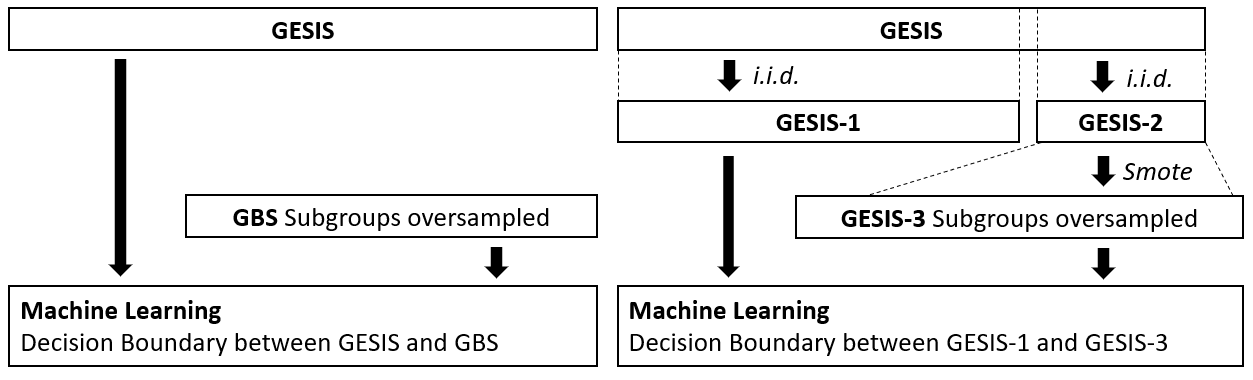
\includegraphics[scale=0.38,angle=0]{fig/procedure2}
		\label{std}
		\caption{Artificial data synthesis to overrepresent subgroups of GESIS. True negatives are removed from the MRS with positive classes GESIS (left) and GESIS-1 (right). Oversampled instances can easily be marked as such for result set comparisons.}
	\end{center}
\end{figure}

The main criterion considered in this work has been the area under the ROC curve. Having a single-number evaluation metric speeds decision-making when selecting among non-representative instances. It gives a clear preference ranking among all of them, and therefore a clear direction for progress. To enable a basis for a more informed exclusion of instances, another important performance criterion generally used in information retrieval could be added. The F-Measure, including summary statistics derived from the precision-recall curve, may be preferred to ROC curves when classes are heavily skewed \cite{jesse}. Precision and recall have been estimated in Section 3 in a positive-unlabeled setting. The area under precision-recall curves \(AUPR\) can be expressed using the approximated value for the fraction of positives \(\alpha\) in \(X_u\): \(\rho = \frac{\alpha \gamma}{\hat{\eta}^{pu}}\).

Lastly, it is up to the research group to analyse political participation and resilience on the given MRS. Table 5.1 evaluates an individual attribute by measuring the amount of information gained about the class "Wahlteilnahme" given the attribute using 10 fold stratified cross-validation. Comparisons of the GBS dataset before and after subsampling might be of interest in this context as well. A closer look at the instances that have been excluded might support the initial claim that people of higher education are over-represented. 

\vspace{0.2cm}
\begin{table}[ht]
      \centering
        \begin{tabular}{lllll}
           Init. avg. merit  & Init. avg. rank &  attribute & MRS avg. merit & MRS avg. rank\\
\hline \hline
	0.164 +/- 0.011 & 1.0 +/- 0.0 & Zufrieden. Wahl. & 0.006 +/- 0.007 & 7.3 +/- 3.5 \\
	0.112 +/- 0.008 & 2.0 +/- 0.0 & Wahlabsicht & 0.096 +/- 0.005 & 1.0 +/- 0.0 \\
	0.040 +/- 0.004 & 3.0 +/- 0.0 & Geburtsland & 0.037 +/- 0.005 & 2.0 +/- 0.0 \\
	0.003 +/- 0.001 & 5.2 +/- 1.3 & Gruppe & 0.002 +/- 0.001 & 3.6 +/- 0.6 \\
        \end{tabular}
\caption{Feature importance in GBS (n=579) and GBS MRS (n=271) for classification of political participation "Wahlteilnahme". In modelling a political participation process, algorithms approximate the likelihood of a person going to vote on election day. Ideally, for every instance with unknown political interest and willingness to participate, there is enough data of people of similiar demographics, socioeconomics and psychological traits to generalize from.}
\end{table}